% !BIB TS-program = biber

\RequirePackage[l2tabu,orthodox]{nag}

% TODO: decide if one-sided/two-sided
%\documentclass[headsepline,footsepline,footinclude=false,fontsize=11pt,paper=a4,listof=totoc,bibliography=totoc,BCOR=12mm,DIV=12]{scrbook} % two-sided
\documentclass[headsepline,footsepline,footinclude=false,oneside,fontsize=11pt,paper=a4,listof=totoc,bibliography=totoc]{scrbook} % one-sided

% TODO: change thesis information
\newcommand*{\getUniversity}{Technische Universität München}
\newcommand*{\getFaculty}{Informatics}
\newcommand*{\getDegree}{Informatics}
\newcommand*{\getSchool}{Computation, Information and Technology}
\newcommand*{\getTitle}{Exploring GPU Programming Models for Autonomous Driving: From Coroutine Integration to Persistent Thread Optimization}
\newcommand*{\getTitleGer}{GPU Coroutines in Autonomes Fahren}
\newcommand*{\getAuthor}{Jaden Rotter}
\newcommand*{\getDoctype}{Bachelor's Thesis}
\newcommand*{\getSupervisor}{Supervisor}
\newcommand*{\getAdvisor}{Jianfeng Gu}
\newcommand*{\getKeywords}{keyword;another keyword;one more}
\newcommand*{\getSubmissionDate}{Submission date}
\newcommand*{\getSubmissionLocation}{Munich}
% TODO: change citation style in settings



\PassOptionsToPackage{table,svgnames,dvipsnames}{xcolor}

\usepackage[a-2u]{pdfx} % generate PDF/A: archival compliant, self-contained pdf
\usepackage[utf8]{inputenc}
\usepackage[T1]{fontenc}
\usepackage[sc]{mathpazo}
%\usepackage[ngerman,american]{babel}
\usepackage[american]{babel}
%\usepackage[ngerman,american,provide=*]{babel}
\usepackage[autostyle]{csquotes}
\usepackage[
  backend=biber,
  style=ieee,
  maxbibnames=99
]{biblatex} 
\addbibresource{bibliography.bib} 
\usepackage{graphicx}
\usepackage{scrhack} % necessary for listings package
\usepackage{listings}
\usepackage{lstautogobble}
\usepackage{tikz}
\usepackage{pgfplots}
\usepackage{pgfplotstable}
\usepackage{booktabs}
\usepackage[final]{microtype}
\usepackage{caption}
\usepackage[printonlyused]{acronym}
\usepackage{ifthen}
\usepackage{float}
\usepackage{listings}
\usepackage{xcolor}
\usetikzlibrary{shadows}
\usetikzlibrary{decorations.pathreplacing, positioning}

\hypersetup{hidelinks} % removes colored boxes around references and links

% for fachschaft_print.pdf
\makeatletter
\if@twoside
	\typeout{TUM-Dev LaTeX-Thesis-Template: twoside}
\else
	\typeout{TUM-Dev LaTeX-Thesis-Template: oneside}
\fi
\makeatother

\addto\extrasamerican{
	\def\lstnumberautorefname{Line}
	\def\chapterautorefname{Chapter}
	\def\sectionautorefname{Section}
	\def\subsectionautorefname{Subsection}
	\def\subsubsectionautorefname{Subsubsection}
}

\addto\extrasngerman{
	\def\lstnumberautorefname{Zeile}
}

% Themes
\ifthenelse{\equal{\detokenize{dark}}{\jobname}}{%
  % Dark theme
  \newcommand{\bg}{black} % background
  \newcommand{\fg}{white} % foreground
  \usepackage[pagecolor=\bg]{pagecolor}
  \color{\fg}
}{%
  % Light theme
  \newcommand{\bg}{white} % background
  \newcommand{\fg}{black} % foreground
}

\bibliography{bibliography}

\setkomafont{disposition}{\normalfont\bfseries} % use serif font for headings
\linespread{1.05} % adjust line spread for mathpazo font

% Add table of contents to PDF bookmarks
\BeforeTOCHead[toc]{{\cleardoublepage\pdfbookmark[0]{\contentsname}{toc}}}

% Define TUM corporate design colors
% Taken from http://portal.mytum.de/corporatedesign/index_print/vorlagen/index_farben
\definecolor{TUMBlue}{HTML}{0065BD}
\definecolor{TUMSecondaryBlue}{HTML}{005293}
\definecolor{TUMSecondaryBlue2}{HTML}{003359}
\definecolor{TUMBlack}{HTML}{000000}
\definecolor{TUMWhite}{HTML}{FFFFFF}
\definecolor{TUMDarkGray}{HTML}{333333}
\definecolor{TUMGray}{HTML}{808080}
\definecolor{TUMLightGray}{HTML}{CCCCC6}
\definecolor{TUMAccentGray}{HTML}{DAD7CB}
\definecolor{TUMAccentOrange}{HTML}{E37222}
\definecolor{TUMAccentGreen}{HTML}{A2AD00}
\definecolor{TUMAccentLightBlue}{HTML}{98C6EA}
\definecolor{TUMAccentBlue}{HTML}{64A0C8}

% Settings for pgfplots
\pgfplotsset{compat=newest}
\pgfplotsset{
  % For available color names, see http://www.latextemplates.com/svgnames-colors
  cycle list={TUMBlue\\TUMAccentOrange\\TUMAccentGreen\\TUMSecondaryBlue2\\TUMDarkGray\\},
}

% Settings for lstlistings
\lstset{%
  basicstyle=\ttfamily,
  columns=fullflexible,
  autogobble,
  keywordstyle=\bfseries\color{TUMBlue},
  stringstyle=\color{TUMAccentGreen},
  captionpos=b
}

\lstdefinelanguage{cuda}{
    language=C++,
    morekeywords={
        __global__, __device__, __host__, __shared__, __constant__,
        cudaMalloc, cudaFree, cudaMemcpy, cudaMemcpyHostToDevice, cudaMemcpyDeviceToHost,
        cudaMallocHost, cudaHostAlloc
    },
    alsoletter={_},
    morekeywords=[2]{int, float, double, bool, void, sizeof},
    morekeywords=[3]{printf, malloc, free},
    keywordstyle=\color{blue}\bfseries,
    keywordstyle=[2]\color{teal}\bfseries, 
    keywordstyle=[3]\color{purple}\bfseries,    
    sensitive=true
}

\lstset{
    language=cuda,
    basicstyle=\ttfamily\small,
    frame=single,
    breaklines=true,
    numbers=left,
    numberstyle=\tiny\color{gray},
    commentstyle=\color{gray},
    stringstyle=\color{orange},
    showstringspaces=false,
    tabsize=2,
    captionpos=b
}

\lstdefinelanguage{x86asm}{
  morekeywords={pushq, popq, movq, ret},
  sensitive=true,
  morecomment=[l]{;},
  morestring=[b]",
}

\lstset{
  language=x86asm,
  basicstyle=\ttfamily\small,
  keywordstyle=\color{blue},
  commentstyle=\color{gray},
  columns=fullflexible,
  keepspaces=true,
  frame=single,
  showstringspaces=false
}


\begin{document}

% Set page numbering to avoid "destination with the same identifier has been already used" warning for cover page.
% (see https://en.wikibooks.org/wiki/LaTeX/Hyperlinks#Problems_with_Links_and_Pages).
\pagenumbering{alph}
\input{pages/cover}

\frontmatter{}

\input{pages/title}
\input{pages/disclaimer}
\addcontentsline{toc}{chapter}{Acknowledgments}
\thispagestyle{empty}

\vspace*{20mm}

\begin{center}
    {\usekomafont{sectioning}\usekomafont{section} Acknowledgments}
\end{center}

\vspace{10mm}

%TODO: Acknowledgments

I want to thank my advisor, Jiangfeng Gu, for overseeing this project and providing the resources that enabled me to explore a topic I am passionate about.
I am grateful for his comments and suggestions, which helped guide my research.
Furthermore, I am grateful to Michael Gerndt, the overseer of this project from his course in Advanced Computer Architecture, which first sparked my interest in GPUs and low-level architecture.
I have greatly benefited from the experience of working on this thesis and look forward to applying these learnings in future projects.

\cleardoublepage{}

\chapter{\abstractname}
This thesis implements a real-time persistent GPU scheduler that can serve as a foundation for a future coroutine and priority-based scheduling implementation.
By keeping threads alive across kernel executions, this approach reduces scheduling overhead and allows tasks to be managed more efficiently and at a finer granularity on the GPU.
Results indicate that these persistent threads are faster and more flexible than traditional kernel launches, making them a promising building block for future coroutine-based programming in areas such as autonomous driving.
These findings highlight the significant impact that low-level GPU scheduling strategies can have on the performance and responsiveness of real-time workloads.


\microtypesetup{protrusion=false}
\tableofcontents{}
\microtypesetup{protrusion=true}

\mainmatter{}

% !TeX root = ../main.tex
% Add the above to each chapter to make compiling the PDF easier in some editors.

\chapter{Introduction}\label{chapter:introduction}
Autonomous driving systems place stringent demands on computational performance and predictability, yet \acsp{GPU}, needed to process sensor data and run machine learning tasks, can not natively support time critical demands. 
The current CUDA \acs{GPU} hardware scheduler, functioning as a black box, maximimizes throughput rather than deterministic execution, leading to unpredictable latency from resource contention, which poses a serious safety hazard.
The proprietary nature of the hardware scheduler makes it difficult to enforce timing guarantees, prioritize critical tasks, and suspend resident kernels.
In the absence of preemption or fine grained resource control, high priority workloads can be delayed by longer running, lower priority kernels. 
This thesis investigates GPU scheduling strategies tailored to real time systems, focusing on GPU coroutines and persistent threads as a mechanism to improve responsiveness, reduce latency variability, and ensure the timely execution of safety critical tasks in autonomous driving.

Early autonomous driving systems used a distributed architecture to ensure the timing guarantees of individual modules \cite{6809196}.
The distributed architecture processes the individual driving tasks into the modules perception, localization, planning, and control, which together form a processing pipeline. 
The stages of the pipeline enable the vehicle to interpret its surroundings, determine its position within them, make decisions, and execute corresponding actions. 
In this architectural design, each module is mapped to an individual compute unit, resolving any resource contention issues between independent modules.
This system design ensures that the load on the compute units is consistent and responsive to the individual modules.
For example, the planning node only ever computes the next, most time critical, planning tasks. 
In this manner, the distributed architecture allows for fine tuning the timing between modules to achieve low latency responses from the hardware. 

Although the system safety was ensured by distributing numerous compute resources, this approach is wasteful and expensive, especially as recent hardware advances in GPUs allow massive cost reduction by centralizing modules onto one processing node.
In addition to the cost and design savings, the intermodule latency is reduced as the results and inputs of different modules are colocated.
This new singular compute node, responsible for all tasks simultaneously, needs to ensure that the execution order respects real time deadlines for the safety of system, passenger and enviornment. 
Despite the centralized architecture being more performant, using a singular compute node risks hardware contention, which can lead to execution latencies. 
Variable execution latencies depending on the execution queue comprimise the system, if GPU tasks can not be preempted to ensure the immediate execution of time critical tasks. 


Unlike \acsp{GPU}, \acsp{CPU} already natively support numerous real time systems at both the OS and programming model levels; however, they currently lack the computational performance needed to meet the strict latency requirements of autonomous driving systems, for which \acsp{GPU} are explicitly required.
The original distributed system design was necessary in part due to the vast amount of computations and processing required by the autonomous driving system.
In particular, the core modules of an autonomous driving system each require complex neural nets in order to allow the vehicle to function autonomously. 
To meet these constraints, autonomous vehicles uses a heterogenous computing architecture with a main CPU, which offloads machine learning and processing work to a specialized processor, such as the NVIDIA \acsp{GPU}. 
The \acsp{GPU} themselves are not designed to be used in real time systems and using standard real time system algorithms for these chips is infeasible due to the different programming models.

Unfortunately, for the same architectural reason as why \acsp{GPU} excell on compute heavy workloads, they can not guarantee execution latencies under task contention. 
NVIDIA \acsp{GPU} are implemented on a batch system algorithm, where throughput is prioritized above all else. 
Unlike real time systems typically implemented on \acsp{CPU}, GPU kernels do not natively support interruption to allow higher priority tasks to execute \cite{taskparallelism}.
The \acs{GPU} kernels are queued and scheduled based on availability and executed until completion without interruption.
By prioritizing throughput over responsiveness and latency, the \acsp{GPU} may become contented between various different tasks, which leads to variable execution and latency times, dependent on the current and queued loads.
Variable latencies are unacceptable in real time systems where strict execution deadlines must be preserved in order to react to the changing enviornment in time. 
This paper proposes a method to allow the \acs{GPU} to be partitioned, reducing kernel launch latency, and enable the integration of \acsp{GPU} into real time systems.


%Background

% !TeX root = ../main.tex
% Add the above to each chapter to make compiling the PDF easier in some editors.
\chapter{Background}\label{chapter:Background}

\section{Integration of GPUs in Autonomous Driving Systems}

Autonomous driving system require \acsp{GPU} for the computational acceleration they provide to the many parallel machine learning models that interpret sensor data, make decisions and ensure safe navigation in real time. 
From perception to planning and control, each stage of the autonomous driving pipeline relies on models that must operate within tight latency constraints. 
These models include convolutional neural networks (CNNs) for image and object recognition, recurrent or transformer-based architectures for temporal sensor fusion and prediction, and reinforcement learning agents or decision trees for behavioral planning \cite{Krizhevsky_undated-ao}.
The sheer diversity and complexity of these tasks require a hardware platform that can execute thousands of operations in parallel in order to achieve the throughput necessary \cite{self_driving_learning}.

GPUs are particularily well suited to these workloads because of their massively parallel architecture and high memory bandwidth, which perfectly meet the demands of deep learning tasks. 
Unlike CPUs, which optimize for sequential instruction execution and low latency branching, GPUs are designed to handle large batches of matrix and tensor operations simultaneously. 
This makes them ideal for real time inference of deep neural networks.
Furthermore, modern GPU architectures provide specialized cores, such as tensor cores in NVIDIA GPUs, that are explicitly optimized for mixed precision matrix multiplication, which is a core operation in most machine learning models. 
By offloading intensive compute tasks to the GPU, autonomous systems can maintain low latency and high accuracy, both of which are crucial for safety and performance in dynamic driving environments.


\section{GPU versus CPU Architecture}
%\cite{taskparallelism} for cuda api not supporting interruption
\acsp{GPU} are capable of delivering this vast increase in throughput over CPUs as measured by GFLOPS, despite the lower clock rate, by simplifying the thread context in order to afford greater parallelism.
They were originally developed to accelerate graphics rendering, a task heavy in parallizable computations, which require only a very simple control overhead and as such have adapted the architecture to support as many possible different threads. 
Typical workloads designed for \acs{CPU} are based on sequential workloads, such as human input or complex logic, which requires complex thread overhead to speed up branches and I/O, through prefetching, branch prediction, and out of order execution.  
These \acsp{CPU} achieve higher single threaded performance by dedicating a "significant portion of transistors to non computational tasks like branch prediction and caching", which \acsp{GPU} can forgo in favor of increasing arithmetic intensity \cite{Owens2007-kp}.
Consider the following graphic Figure~\ref{fig:thread_complexity}, which highlights the difference in thread complexity. 


%This choice in architectural design makes \acsp{GPU} excell on data processing and machine learning workloads due to thier

%Both data processing and machine learning tasks rely extensively on intensive matrix computations, which can be easily parallelized.
%These tasks benefit, both in processing speed and model complexity, from the \acs{GPU}'s ability to perform thousands of operations in parallel, far greater than the traditional \acs{CPU} can achieve.

%\section{\acs{GPU} Limitations in Real Time Systems}

%\subsection{GPU vs CPU Threads}

%\acsp{GPU} have parallelised the thread centric scheduling execution model on \acsp{CPU} to reflect the architectural design.  
%\acsp{CPU} schedule threads to execute

%The fundamental differences betweeReal time systems \acs{GPU} threads differ significantly from \acs{CPU} threads, esulting
%To maximize computational and energy efficiency at scale, \acsp{GPU} maintain a minimal thread context in comparison to \acsp{CPU}. 
%\acsp{CPU} are engineered for general-purpose computing, where performance often involves improving single threaded execution.
%Achieving higher single-threaded performance means dedicating a "significant portion of transistors to non-computational tasks like branch prediction and caching" \cite{Owens2007-kp}.
%Instead, \acsp{GPU} sacrifice this complex control overhead to save transistors, which can be used for increasing the arithmetic intensity capability.
%This architectural choice is illustrated in Figure\Figure~\ref{fig:thread_complexity}, which highlights how the \acs{GPU}’s simplified control logic reduces overhead, allowing more transistors to be used for arithmetic units \cite{Owens2007-kp}.

\begin{figure}[htbp]
  \centering
  \resizebox{1.0\linewidth}{!}{
    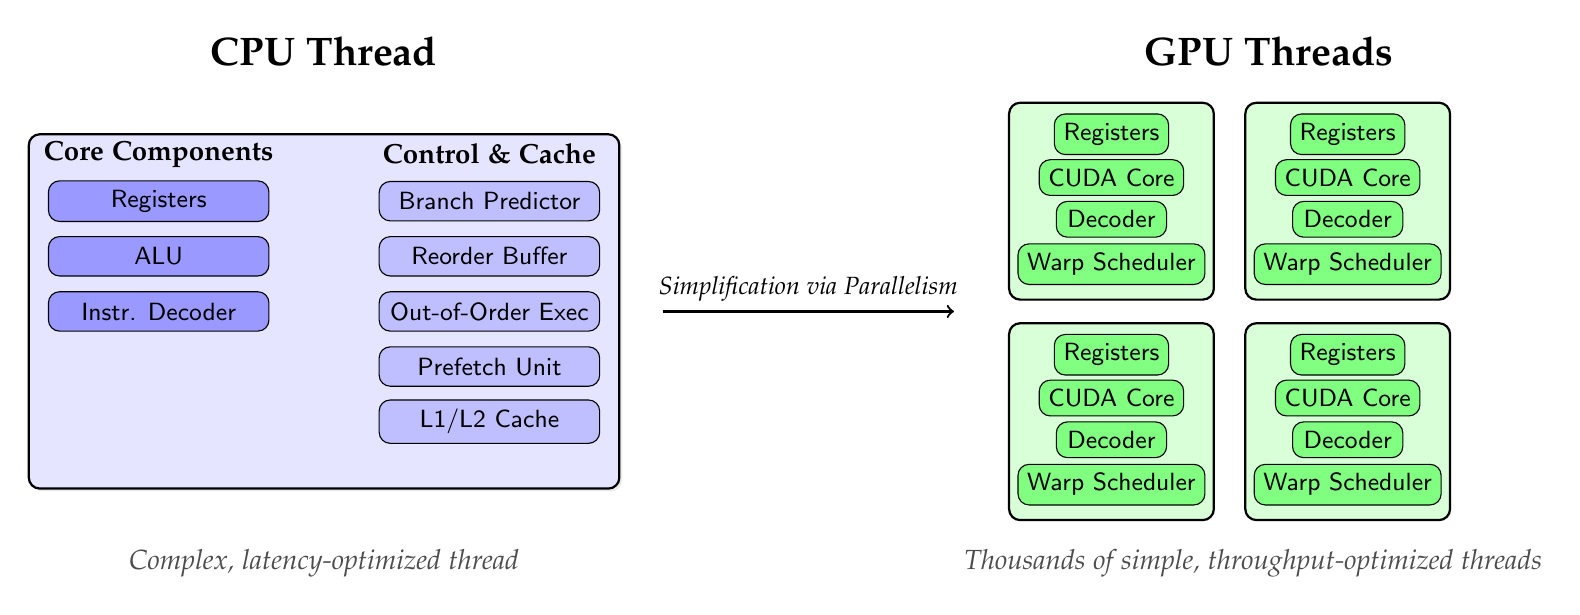
\begin{tikzpicture}[font=\sffamily\small]
% === CPU THREAD BLOCK ===
\begin{scope}[xshift=0cm, yshift=0cm]
    % Main CPU thread container with shadow
    \node[draw, thick, rounded corners, minimum width=7.5cm, minimum height=4.5cm, fill=blue!10, drop shadow={shadow xshift=1pt,shadow yshift=-1pt,opacity=0.15}] (cpuBox) {};

    % Group titles
    \node[font=\bfseries] at (-2.1, 2.0) {Core Components};
    \node[font=\bfseries] at (2.1, 2.0) {Control \& Cache};

    % Left side shared components
    \node[draw, fill=blue!40, minimum width=2.8cm, minimum height=0.5cm, rounded corners, align=center] at (-2.1,1.4) {Registers};
    \node[draw, fill=blue!40, minimum width=2.8cm, minimum height=0.5cm, rounded corners, align=center] at (-2.1,0.7) {ALU};
    \node[draw, fill=blue!40, minimum width=2.8cm, minimum height=0.5cm, rounded corners, align=center] at (-2.1,0.0) {Instr. Decoder};

    % Right side CPU-only components
    \node[draw, fill=blue!25, minimum width=2.8cm, minimum height=0.5cm, rounded corners, align=center] at (2.1,1.4) {Branch Predictor};
    \node[draw, fill=blue!25, minimum width=2.8cm, minimum height=0.5cm, rounded corners, align=center] at (2.1,0.7) {Reorder Buffer};
    \node[draw, fill=blue!25, minimum width=2.8cm, minimum height=0.5cm, rounded corners, align=center] at (2.1,0.0) {Out-of-Order Exec};
    \node[draw, fill=blue!25, minimum width=2.8cm, minimum height=0.5cm, rounded corners, align=center] at (2.1,-0.7) {Prefetch Unit};
    \node[draw, fill=blue!25, minimum width=2.8cm, minimum height=0.5cm, rounded corners, align=center] at (2.1,-1.4) {L1/L2 Cache};

    % CPU label
    \node[font=\itshape, text=black!70] at (0,-3.2) {Complex, latency-optimized thread};
\end{scope}


% === GPU THREAD GRID ===
\begin{scope}[xshift=10cm, yshift=-1.4cm]
    % 2x2 Grid of simple GPU threads
    \foreach \x in {0,1} {
        \foreach \y in {0,1} {
            \begin{scope}[xshift=3.0*\x cm, yshift=2.8*\y cm]
                % Single GPU thread block
                \node[draw, thick, rounded corners, minimum width=2.6cm, minimum height=2.5cm, fill=green!15, drop shadow={shadow xshift=0.5pt,shadow yshift=-0.4pt,opacity=0.1}] {};

                \node[draw, fill=green!50, minimum width=1.4cm, minimum height=0.35cm, rounded corners, align=center] at (0,0.85) {Registers};
                \node[draw, fill=green!50, minimum width=1.4cm, minimum height=0.35cm, rounded corners, align=center] at (0,0.3) {CUDA Core};
                \node[draw, fill=green!50, minimum width=1.4cm, minimum height=0.35cm, rounded corners, align=center] at (0,-0.23) {Decoder};
                \node[draw, fill=green!50, minimum width=1.4cm, minimum height=0.35cm, rounded corners, align=center] at (0,-0.80) {Warp Scheduler};
            \end{scope}
        }
    }

    % GPU label
    \node[font=\itshape, text=black!70] at (1.8, -1.8) {Thousands of simple, throughput-optimized threads};
\end{scope}


% === Titles ===
\node[font=\Large\bfseries] at (0,3.3) {CPU Thread};
\node[font=\Large\bfseries] at (12.0,3.3) {GPU Threads};


% === Arrow between CPU and GPU ===
\draw[->, thick] (4.3,0.0) -- (8.0,0.0) node[midway, above, font=\small\itshape] {Simplification via Parallelism};

\end{tikzpicture}

  }
  \caption{CPU vs GPU Thread Architecture}
  \label{fig:thread_complexity}
\end{figure}


Although core components are named differently, both CPU and GPU threads work fundamentally similarily with an instruction decoder, registers and an arithmetic unit. 
The differences arise when trying to maximize a single control flow. 
The CPU will prefetch instructions, reorder them to most effectively use the functional units and speculatively compute instructions based on a branch predictor. 
On the other hand, \acs{GPU} threads can not execute instructions out-of-order, use only manual prefetching, and have a simple branch predictor that is far more conservative than the \acs{CPU}'s predictor.
Furthermore, the \acs{GPU} amortisizes the cost of managing an instruction stream accross multiple threads, which execute the same instructions at the same time versus the \acs{CPU} execution model which 
The additional complex logic involved allows single threaded \acs{CPU} applications to far outperform single threaded GPU applications, as seen by the following comparison of single threaded matrix multiplication in Figure~\ref{fig:singlethreadedgraph} and Figure~\ref{fig:singlethreadedmatrix}.

\begin{figure}[H]
  \centering 
  \resizebox{1.0\linewidth}{!}{
	  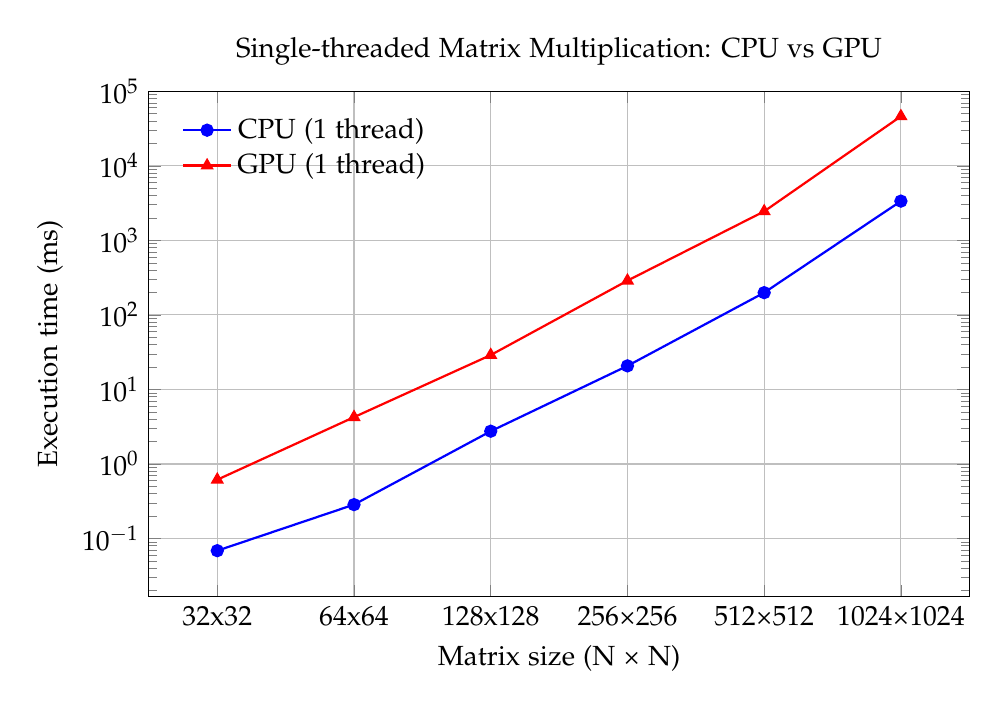
\begin{tikzpicture}
\begin{axis}[
    ymode=log,
    log basis y=10,
    width=12cm,
    height=8cm,
    xlabel={Matrix size (N × N)},
    ylabel={Execution time (ms)},
    title={Single-threaded Matrix Multiplication: CPU vs GPU},
    legend pos=north west,
    xtick=data,
    xticklabels={32x32, 64x64, 128x128, 256×256, 512×512, 1024×1024},
    ymin=0,
    ymax=100000,
    grid=major,
    legend style={draw=none, fill=none}
]

\addplot+[mark=*, thick, blue] coordinates {
    (1, 0.068705)
    (2, 0.285104)
    (3, 2.751817)
    (4, 20.706290)
    (5, 198.716200)
	(6, 3356.762000)
};
\addlegendentry{CPU (1 thread)}

\addplot+[mark=triangle*, thick, red] coordinates {
    (1, 0.615584)
    (2, 4.249685)
    (3, 28.923530)
    (4, 287.943700)
    (5, 2446.466000)
    (6, 46097.410000)
};
\addlegendentry{GPU (1 thread)}

\end{axis}
\end{tikzpicture}

  }
  \caption{Single threaded Matrix Multiplication Execution between CPUs and GPUs averaged over 10 executions}
  \label{fig:singlethreadedgraph}
\end{figure}

\begin{figure}[H]
	\centering
	\resizebox{1.0\linewidth}{!}{
		\begin{tabular}{|r|r|r|r|r|}
\hline
\textbf{Matrix Size (n $\times$ n)} & \textbf{CPU Time (ms)} & \textbf{GPU Time (ms)} & \textbf{Speedup (GPU/CPU)} \\
\hline
32 $\times$ 32     & 0.068705   & 0.615584    & 11.970438 \\
64 $\times$ 64     & 0.285104   & 4.249685    & 15.554119 \\
128 $\times$ 128   & 2.751817   & 28.923530   & 11.419879 \\
256 $\times$ 256   & 20.706290  & 287.933700  & 13.906730 \\
512 $\times$ 512   & 198.716200 & 2446.466000 & 12.323010 \\
1024 $\times$ 1024 & 3356.762000 & 46097.410000 & 13.745850 \\
\hline
\end{tabular}


	}
	\caption{Data Matrix from Figure~\ref{fig:singlethreadedgraph}}
	\label{fig:singlethreadedmatrix}
\end{figure}	




As seen in Figure~\ref{fig:singlethreadedgraph} and Figure~\ref{fig:singlethreadedmatrix} applications that fail to utilize the concurrancy of \acsp{GPU}, either due to programmatical errors or a lack of parallelism in the task, will struggle to achieve high performance.
For each of the matrices tested, through prefetching, a higher clock rate, and branch prediction, the CPU is on average around 13 times faster than the \acs{GPU} running the exact same algorithm. 
Following these results, the \acs{GPU} should only be used in place of the \acs{CPU}, when the application is well tuned to the programming model and a scheduler must respect this difference.
If a \acs{GPU} scheduler is written without regard for these differences, it will may not be able to achieve the desired performance benefit.
This fundamental architectural and programming style for \acsp{GPU} must be understood in order to maximize the throughput. 

\subsection{GPU Hardware Architecture based on the Tesla V100 GPU\footnote{For the purpose of this thesis, the NVIDIA Tesla V100 GPU chip, which uses the Volta GV100 architecture, was selected due to its availability and high performance computing capabilities.}}


For the purposes of programming and scheduling tasks onto the Tesla V100 GPU, the GPU appears as an array of independent highly parallelized processors, called \acsp{SM}.
The \acsp{SM} are grouped into specific \acsp{TPC}, which are then further grouped into \acsp{GPC}, but the specific mapping of tasks to \acs{SM}, \acs{TPC}, and \acs{GPC} is determined by the proprietary hardware scheduler, the GigaThread Engine. 
The exact workings and scheduling methods of the GigaThread Engine are not publicly available, but this module maps \acsp{CTA}, groups of threads executing the same instruction code, to the individual \acsp{SM} based a multitude of factors: hardware resources, parallelism, priorities, and dependencies.
Similarily, the global memory and L2 cache utilization are determined by the hardware and transparent to the programmer.
After the \acs{CTA} gets mapped to the specific \acs{SM}, the device code then executes till completion. 
Each \acs{SM} manages its scheduled \acsp{CTA} through its own execution pipelines, register files, shared memory and scheduling units that function independently from one another. 
For \acsp{SM} to communicate with one another, they must use either the global on-chip device \acs{HBM2} or through the global L2 cache which is shared and coherent across all \acsp{SM}.
Although these memory accesses allows individual \acsp{SM} to communicate with each other, accesses require hundreds of cycles, which introduce further latencies when compared to local \acs{SM} L1 memory caches.
Ideally, the \acsp{SM} execute independently of one another and cumulate answers in global memory, skipping the high memory latency accesses of coordinating synchronous work.

Applications are scheduled to the \acs{SM} by the GigaThread Engine consisting of a \acs{CTA}, or block of threads executing the same instruction code, which then get subdivided into warps to be executed across the \acs{SM}'s execution units.
On the \acs{GPU}, the smallest unit of execution is the Warp, a group of 32 threads that executes instructions in lockstep.
Warps always consist of 32 threads, even if the \acs{CTA} is not divisible by 32 and cannot be fully partitioned across the warps. 
The lockstep execution pattern of warps, enforce that each thread within the warp executes the same instruction, even if several threads are inactive. 
As a consequence, control logic that forces divergent threads significantly slows execution and overutilizes CUDA cores, as the individual threads are forced to execute sequentially.
%If the \acs{CTA} is scheduled with a number of threads indivisible by 32, then the last Warp will still have 32 threads, but the additional threads are deactiveated using a mask.
%Consider the implementation of a program with 33 threads. 
%This application would use 33 software threads, but take up 64 hardware threads with most the CUDA cores assigned by the dispatch unit in the second Warp sitting idle, while the only active thread executes. 

The Tesla V100 GPU \acs{SM} architecture, self contains an entire execution pipeline within each of its 4 processing partitions, which collectively share an L1 instruction cache as well as an L1 data and shared memory cache.
As \acsp{CTA} are distributed across multiple Warps, these collective L1 caches allow the instruction memory and shared memory to be stored across different Warps within the same \acs{CTA}.
The main components of each processing partition are a L0 instruction cache, warp scheduler, dispatch unit, execution units.
Every clock cycle, the Warp scheduler schedules a singular Warp of 32 threads, which get passed to the Dispatch unit. 
The dispatch unit then dispatches a new instruction to the Warp every clock cycle. 
As for any given instruction there are not enough execution units of the same type, the instructions get queued onto the execution units. 
Depending on the current queue and any delays, such as global memory accesses or dependencies, the Warp scheduler will interweave different Warps together onto the Dispatch Unit to hide latencies. 
Within each \ac{SM} processing partition's execution units, there are Tensor Cores for deep learning, 64 bit-\ac{FP} cores, \ac{LD/ST} units, a register file, and \acs{SFU}s for mathematical functions such as sine and square root. 
An in depth view of the processing partition's architecture is provided in Figure~\ref{fig:processing_partition}.



\begin{figure}[H]
  \centering
  \includegraphics[width=0.3\textwidth]{figures/output-006.png}
  \caption{Architecture from the whitepages: https://images.nvidia.com/content/volta-architecture/pdf/volta-architecture-whitepaper.pdf}
  \label{fig:processing_partition}
\end{figure}

A \ac{SM} can support up to 64 concurrent warps, allowing a maximum of $64 * 32 = 2048$ threads per \ac{SM}. 



\acsp{GPU} have revolutionized data processing and machine learning training and inference with their ability to handle massive amounts of data and execute simple, but highly-parallelized computations.
Data processing systems, based on traditional CPUs, rely on a \ac{MIMD} architecture that excels at handling complex control logic at high frequencies by executing different instructions on seperate data streams concurrently. 
However, for  tasks that require the repeated execution of singular instructions such as large-scale data processing workloads, \acsp{CPU} are burdened by the overhead of the complex control logic, where a simpler, more parallel design would be more effective.
\acs{GPU}s, created to overcome this limitation, use a \ac{SIMT} architecture with thousands of simpler, but slower threads executing simultaneously. 
% TODO
For example, the current architecture generally supports as many as 2048 threads in a single block, which can run on a single \ac{SM}, scaling the number of concurrent threads by the number of \acsp{SM}, by the number of \acsp{SM}, 80 on the newer models. 
% TODO
The parallelism provided by the \ac{SIMT} model allows a far higher throughput that outperforms \acsp{CPU}. 
Here, each data element is processed by its own thread, allowing the same instruction to be executed simultaneously across numerous data streams.

% TODO
Real time systems, which rely extensively on machine learning tasks and data processing tasks, Higher data processing performance is vital to autonomous systems, which rely extensively on machine learning tasks and sensor data processing. 
In autonomous systems a multitude of modules require deep learning, a machine learning technique, to automatically extract patterns, such as computer vision, and make decisions \cite{JEON2021167}.
Deep learning, inspired by the structure of the human brain, is composed of layers of numerous interconnected, identical nodes called neural networks.  
Neural network models rely on mathematical operations between different neighboring layers to perform inference, essentially the prediction making or recognition process.
The layers are represented as matrices, which then get multiplied and convoluted with one another and are used by specialized functions, called activation functions, to introduce non-linearity. 
With very large neural networks with thousands or millions of nodes, the inference computation is repetitive and slow. 
The capability to execute these repeptitive workloads concurrently across different dataset makes \acsp{GPU} fundamental to performance in tasks using complex neural networks.  
Furthermore, \acsp{GPU} are necessary to process the data rate produced by high-bandwidth, high-frequency sensors used in autonomous driving. 
The parallelism in \acs{GPU}s makes them the ideal platform over CPUs for deep learning and data processing tasks, tasks fundamental for autonomous driving systems.


Real time systems, such as autonomous driving, are designed with strict timing constraints in mind, to ensure predictable and deterministic behavior \cite{10155700}. 
deadlines, which are subdivided into soft and hard-deadlines. 
Hard deadlines are critical and a failure leads to the systems failure or unsafe conditions. 
For example, in autonomous driving, collision avoidance with another vehicle and brake activation are hard deadlines. 
If these deadlines are not met, the safety of the passengers and the system is at risk. 
On the other hand, soft deadlines are not critical and missing these deadlines degrades performance, but does not cause system failure. 
In autonomous driving, this would show in route planning and navigation updates, where a delay would lead to suboptimal paths, but safety is not comprimised. 
Real time systems need to be capable of effectively and efficiently switching from lower priority tasks, soft deadline tasks, to high priority, hard deadline tasks, to ensure the safety both for the passengers and nearby individuals.  





\subsection{Necessesity of \acsp{GPU} in Autonomous Driving}

\subsection{Autonomous Driving as a Real Time System}

\section{Background}
\subsection{Asynchronous Programming and Coroutines}

Asynchronous programming is a method of programming a system to handle tasks concurrently instead of sequentially. 
Typically used in conjunction with tasks that delay or have high wait-times, such as I/O heavy jobs, asynchronous programming reduces overall execution time by more efficiently using processing ressources. 
For example, while waiting for I/O heavy input like sensor I/O, asynchronous code lets other tasks execute in the meantime, before returning when the data arrives.  
For real-time systems, asynchronous programming additionally uses the intermittant execution model to enforce determinism. 
By allowing the \acsp{GPU} to switch between concurrent tasks, hard deadlines can be immediately enforced without delay. 


Coroutines, an implementation of asynchronous programming, uses suspendable functions to halt execution. 
Suspendable functions are implemented by capturing the current context, know as the continuation, of the currently running thread and save the data to be run later \cite{Zheng2022LuisaRender}. 
After being saved, a new process can take over execution, without interrupting or overwritting the state of the previous process. 
Once the intermittant process or higher priority process has finished execution, the original task can continue executing by restoring the process context, which was previously saved. 
Capturing the continuation of a function allows the resumption of the program to be strategically deferred. 

%Here, the scheduled tasks are independent of the control flow, meaning the execution order of the subtasks





\subsection{NVIDIA Tesla V100 Architecture}


 %\section{Motivation}
 %In autonomous driving and other real time system tasks, GPUs are essential for data processing and machine learning; however,  existing GPU scheduling techniques fail to meet the strict timing requirements of real-time applications.
 %GPU tasks are traditional queued and scheduled based on availabilty to optimize for high throughput applications like graphics rendering and offline machine learning training.
 %These tasks run to completion before switching tasks, meaning multiple tasks, such as the different modules in autonomous driving cannot efficiently share resources. 
 %Depending on the current workload for the GPU, execution times and latency can vary. 
 %These limitations make existing GPU scheduling mechanisms unsuitable for real-time applications like autonomous driving, where deadlines need to be met to ensure the safety of the system and passengers. 

%Citation test~\parencite{latex}.

%Acronyms must be added in \texttt{main.tex} and are referenced using macros. The first occurrence is automatically replaced with the long version of the acronym, while all subsequent usages use the abbreviation.

%E.g. \texttt{\textbackslash ac\{TUM\}, \textbackslash ac\{TUM\}} $\Rightarrow$ \ac{TUM}, \ac{TUM}

%For more details, see the documentation of the \texttt{acronym} package\footnote{\url{https://ctan.org/pkg/acronym}}.




%Autonomous driving system

%In order to react in time to input, autonomous driving systems need to efficiently process 

%By removing human error and utilizing the faster reaction times of computers, autonomous driving can make transportation safer, more accessible, improve traffic efficiency, and reduce the number of traffic accidents.

%For \ac{AVs}, driving tasks rely on complex computations to both understand the surrounding environment and to react to it in real-time.
%Many of these computations are scheduled onto a \ac{\ac{GPU}}, to leverage the high degree of parallelism in the architecture. 
%However, similar to \ac{CPU}s, the \ac{\ac{GPU}} can experience contention when multiple tasks compete for processing power. 
%Unlike \ac{CPU}s, though, \ac{\ac{GPU}}s are less efficient at quickly switching between different tasks, which can lead to delays and unpredictability. 
%If too many tasks get scheduled at once, the system's ability to meet critical deadlines can be comprimised, potentially leading to safety hazards. 
%Using coroutines on persistant threads, \ac{\ac{GPU}} scheduling can be adapted to mitigate contention and ensure real-time system guarantees, enhancing the safety and reliability of \ac{AV}s.


%These autonomous driving modules use vast amounts of data for their computation tasks, which are based in deep learning, a machine learning technique that demands vast amounts of computational resources.
%Deep learning, inspired by the structure of the human brain, utilizes neural networks, with many layers of neural nodes, to automatically extract patterns, enabling decision-making tasks such as classification and object detection.  
%In perception, deep learning models, particularily \acs{CNN}s identify objects, lane markings, pedestrians, vehicles, and traffic lights from the raw sensor data. 
%Beyond perception, deep learning enhances localization by refining sensor fusion techniques, improving accuracy in determining the vehicles position. 
%Furthermore, deep learning also supports planning and control, through reinforcement learning and predictive models to optimize trajectories. 
%The real-time nature of these components are needed to reduce the latency, which requires these models to continously be updating their predictions as new sensor input arrives and the vehicle moves.
%This places a high demand on the hardware, requiring high-performance accelerators to process vast amounts of data efficiently. 
%To meet these requirements, these computations are scheduled on to a \ac{GPU}, which provides the high degree of parallelism required by the vast amount of data and computations within autonomous driving. 



Real time systems, such as autonomous driving, are designed with strict timing constraints in mind, to ensure predictable and deterministic behavior \cite{10155700}. 
They use a concept of deadlines, which are subdivided into soft and hard-deadlines. 
Hard deadlines are critical and a failure leads to the systems failure or unsafe conditions. 
For example, in autonomous driving, collision avoidance with another vehicle and brake activation are hard deadlines. 
If these deadlines are not met, the safety of the passengers and the system is at risk. 
On the other hand, soft deadlines are not critical and missing these deadlines degrades performance, but does not cause system failure. 
In autonomous driving, this would show in route planning and navigation updates, where a delay would lead to suboptimal paths, but safety is not comprimised. 
Real time systems need to be capable of effectively and efficiently switching from lower priority tasks, soft deadline tasks, to high priority, hard deadline tasks, to ensure the safety both for the passengers and nearby individuals.  

% !TeX root = ../main.tex
% Add the above to each chapter to make compiling the PDF easier in some editors.

\chapter{Objectives}\label{chapter:Objectives}

The objective for this thesis is to develop, implement and evaluate a persistant thread with coroutine based scheduling approach for GPU threads in Apollo\footnote{Apollo is an open-source project developed by Baidu. For more information, visit the GitHub repository: \url{https://github.com/ApolloAuto/apollo}}, an open source autonomous driving platform, to improve real-time safety and determinism by ensuring a predictable scheduling behavior. 
This requires analyzing the limitations of existing GPU scheduling techniques, which, due to their batch processing design, lack the ability to perform task switching. 
To adress this, the new coroutine based scheduling mechanism LuisaCompute-coroutine\footnote{\cite{Zheng2022LuisaRender} and the accompanying source code \url{https://github.com/LuisaGroup/LuisaCompute-coroutine/tree/next}} will be employed. 
The Luisa coroutine scheduling was designed for graphics rendering tasks, around which their \ac{DSL} is written. 
Therefore, the scheduler and its \ac{DSL} will need to be adapted to fit the requirements of the autonomous driving domain, which prioritizes responsiveness, fault tolerance, and strict timing guarantees.  
By integrating this feature into Apollo, the GPU will be able to use coroutines for more flexible and efficient task management, ultimately enhancing the reliability and safety of the real-time autonomous driving platform.  

\subsection{Measurement and Evalutation}

To measure the success of a coroutine based solution, the latency of new time sensitive task scheduling and deadline success will be evaluated in comparison to the old system.
Furthermore, the implementability and effectiveness of this application will be analyzed through practical experiments and benchmarks, focusing on how well the system maintains deterministic behavior under varying workloads and task complexity. 


	

\section{GPU Programming Models for Real Time Systems}\label{chapter:Coroutines}

In order to meet urgent deadlines, systems need to prioritize and ensure the timely execution of critical tasks.
Prioritizing execution requires that high priority tasks are scheduled first when resources are available, and that their deadlines are still met even when resources are fully occupied. 
Achieving this responsiveness, requires preemption or context switching between resident tasks and scheduled critical tasks. 
In Apollo, this responsiveness is implemented through coroutines, which cooperatively yield execution to enable timely task switching.
Coroutines are particularly well suited to GPU scheduling, since GPUs lack integrated hardware preemption and therefore depend on cooperative mechanisms to maintain responsiveness.


\subsection{Coroutines}

Coroutines are a form of asynchronous programming that enables cooperative multitasking between functions.
Unlike traditional thread or process switches, which can occur at any time and requires a larger context, coroutine switches happen only at programmer defined suspension points. 
This makes them particularly useful for enabling runtime kernel task switching on the GPU. 
Here, execution of a kernel can be suspended to allow another kernel to run, and then later resumed without blocking other work.

A coroutine suspends execution by capturing its current context, known as the continuation, which contains the execution state needed for later resumption \cite{Zheng2022LuisaRender}.
Once suspended, another task can execute without overwriting or disrupting the saved kernel state.
When the interim task completes, the coroutine can continue exactly where it left off by restoring its continuation.
This ability to strategically pause and resume execution makes coroutines well suited for real time workloads, where rapid switching between concurrent tasks can help meet hard deadlines without delay.


\subsubsection{CPU Coroutines in Apollo}

Coroutines on the CPU are implemented using the native x86 calling conventions and the program stack to dynamically save and restore continuations.
Under x86 convention, when a function is invoked, the CPU pushes the return address, the location after the next instruction after the call, onto the stack before jumping to the target function.
The called function accesses its local variables through the stack and registers, which are divided into two categories, volatile, caller saved and non volatile, callee saved.
Volatile registers may be freely modified by the callee, while callee saved registers must be preserved and restored before the function returns.

When excecution reaches a return instruction, the CPU pops the return address off the stack and continues execution from that point.
To implement coroutine behaviour, however, the function must be able to yield and later resume.  
This requires saving the callee saved registers, since thier preservation is guaranteed, as well as any additional state such as local variables or registers, that is necessary for continued execution.
These elements can be stored on the stack, enabling a coroutine to pause and later continue seamlessly. 

The Apollo project demonstrates this mechanism with CPU coroutines implemented directly on top of the x86 calling convention, as illustrated in the following example. 

\begin{lstlisting}[language=x86asm,caption={CPU Coroutine}, label={lst:coro}]
ctx_swap:
    pushq %rdi
    pushq %r12
    pushq %r13
    pushq %r14
    pushq %r15
    pushq %rbx
    pushq %rbp
    movq %rsp, (%rdi)

    movq (%rsi), %rsp
    popq %rbp
    popq %rbx
    popq %r15
    popq %r14
    popq %r13
    popq %r12
    popq %rdi
    ret
\end{lstlisting}

The CPU coroutine implementation uses the context switching function, ctx\_swap, which captures the current continuation and restores the state of another coroutine. 
This function accepts two parameters, \texttt{\%rdi} and \texttt{\%rsi}, which point to the memory locations used to store and retrieve coroutine continuations.
Execution happens in two stages.
In the first stage, the continuation is stored and its address is saved to the register \texttt{\%rdi}.  
The second stage then moves the stack frame to the location of its continuation, using the register \texttt{\%rsi}, before restoring the new coroutine context.

Each stage loads or saves their registers in a specific defined order. 
In particular, to ensure the memory is reread into the correct registers, the order of pushing elements onto the stack is the reverse order of popping elements. 
As the stack works on a last in first out principle, this ensures that all the registers have the correct values upon resumption. 
In comparison to traditional context switches involving processes or threads, coroutine context switching via ctx\_swap operates with significantly lower overhead, resulting in faster execution.

\subsection{GPU Coroutines}

Unlike CPU coroutines, which can implement context switching by saving and restoring stack frames, GPUs cannot use the same mechanism, as GPU threads do not maintain conventional stack frames.
Instread, their execution state is managed differently, requiring specialized approaches to preserve and resume coroutine execution.

Attempting to implement CPU style coroutines using the ctx\_swap function does not work because GPUs handle function calls differently.
\acsp{CPU} stores a call stack of function stack frames, which can be easily accessed and manipulated by pushing and popping values or addresses.
\acsp{GPU}, in contrast, avoids traditional stack frames by aggressively inlining function calls, reducing overhead since function code is readily available and no stack frame is needed. 

Implementing and manipulating deep call stacks on GPUs is largely handled by the compiler and hardware, leaving very little control to the programmer, which makes such approaches impractical.
For example, CUDA originally did not support recursive functions, which were only introduced later via the \lstinline[language=cuda]`-rdc=true` flag. 
Even then, recursion comes with strict limitations on stack size and adds significant performance overhead.
Attempting to rely on deep call stacks can quickly lead to excessive instruction and register usage, illustrating why GPU architectures and compilers discourage CPU style stack manipulation.

\subsubsection{Persistent Threads to support Coroutines}

Given that call stacks are not effectively or efficiently supported in CUDA, the GPU needs to support a user level runtime scheduling mechanism to manage the contexts dynamically. 
Due to the nature of kernels executing until completion, the \acs{GPU} coroutine scheduler needs to be based on a persistent kernel, which can schedule coroutines throughout the lifetime of the application.
The coroutines running on the persistent threads will then define suspension points to manually give control back to the scheduler in order to switch tasks. 
Because storing every register for all threads across coroutines is too expensive and inaccessible, coroutine contexts must be explicitly synthesized and saved in global memory, freeing the limited \acs{SM} resources for new tasks.

\subsection{Persistent Kernels}

Persistent GPU threads give the programmer enhanced control over hardware scheduling by running on top of the hardware scheduler, enabling manual execution decisions that are otherwise unavailable.  
In addition to this increased flexibility, persistent kernels reduce runtime scheduling overhead.
As the hardware resources are preallocated, thread and block configurations are loaded ahead of execution, the runtime avoids repeatedly configuring these settings, allowing kernels to run more efficiently. 
In systems with recurring or periodic tasks, such as autonomous driving, this overhead becomes particularly costly. 
With the implementation of persistent threads, only input and output buffers need to be updated for each new task, minimizing execution overhead and allowing kernels to operate with only the essential arguments required for computation.





% !TeX root = ../main.tex

\chapter{Design and Implementation Requirements}\label{chapter:Persistent Threads}

Persistent GPU threads allow the hardware resources to be partitioned and reduce kernel execution and scheduling overhead and are fundamental for other applications seeking to enhance GPU scheduling.  
Many other applications such as coroutines or mega kernels are based on persistent threads as a means of reducing kernel launch overhead and allow further control in application specific scheduling decisions, otherwise black boxed by the cuda api. 
Running persistent threads essentially allows the memory and system configurations to be loaded in ahead of runtime and reduces overhead during execution.

Failing to implement LuisaCompute's coroutines into Apollo, the goal shifted to finding a manual GPU scheduling functionality to implement and use. 
In restricting the scope from GPU coroutines to simply implementing persistent threads into Apollo, this thesis attempted to find an open source implementation which would allow the fine grained scheduling controll specific to Apollo. 
Unfortunately, given that most persistent thread implementations are highly specific they are not open source, which led to selecting an implementation that required more work to make it feasible. 
The only open source persistent thread implementation that was readily available was LightKer, a research project, which measured the hypothetical speedup of using persistent threads over sequential kernel launches. 
Seeking to implement LightKer into Apollo first required a complete restructuring of the code base to support a real time system.

The LightKer implementation itself intended to measure the performance difference between sequential kernel executions versus a persistent kernel implementation.
This implementation constructed simple trivial kernels and tested the overhead difference between calling them explicitely from the host in kernel launches versus implicitely in the persistent kernel. 
Unfortunately, this application does not support variable tasks or memory transfers at runtime, necessary to pass arguments and results back and forth. 
As such, the implementation only succeeds in measuring latency differences between scheduling tasks using a device side while loop versus explicit kernel launches. 
However, the LightKer implementation does provide a simple framework for using a GPU-Host mailbox for scheduling kernel tasks as well as a helpful persistent kernel launch structure. 

\section{Architecture}

From a high level, the architecture implemented into this project appears as follows, with the GPU-Host Mailbox, being used from the Lightkernel project as well as the internal structure.

\begin{figure}[H]
  \centering
  \resizebox{1.0\linewidth}{!}{
	  %\documentclass[tikz, border=5mm]{standalone}
%\usepackage{tikz}
%\usetikzlibrary{shapes, arrows.meta, positioning, decorations.pathreplacing}

%\begin{document}

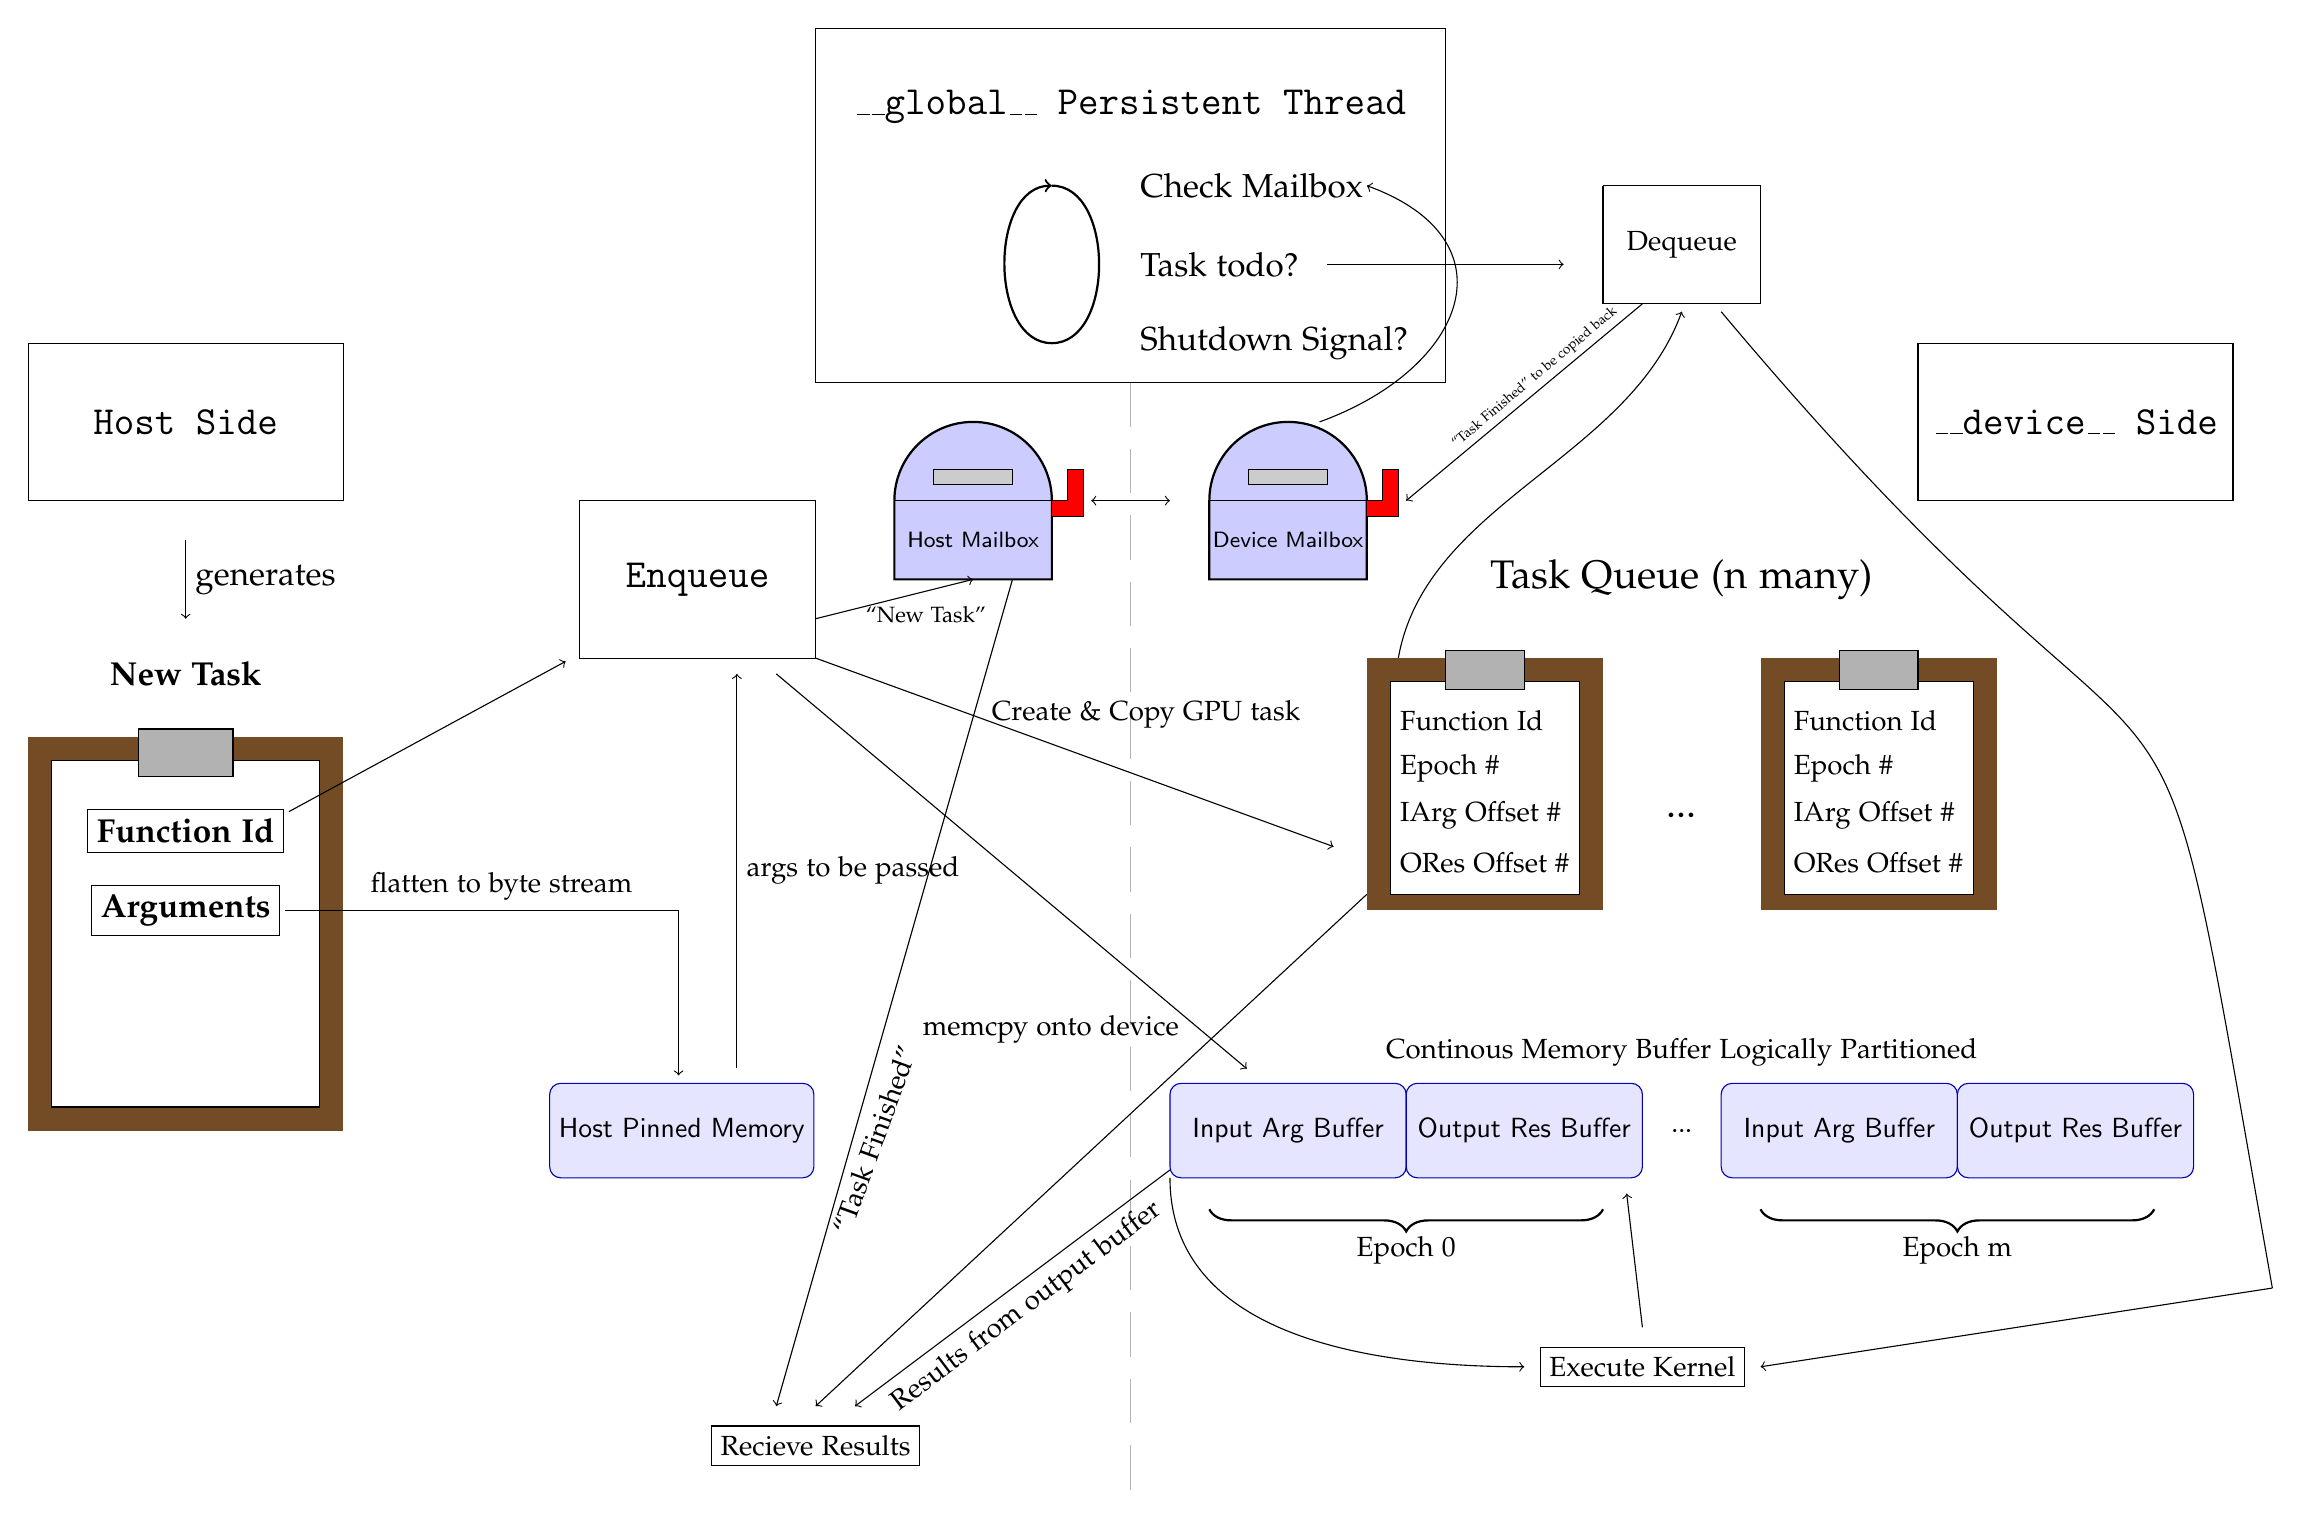
\begin{tikzpicture} [memoryblock/.style={
		draw=blue!70!black, 
		fill=blue!10, 
		rounded corners=4pt, 
		minimum width=3cm, 
		minimum height=1.2cm,
		font=\sffamily
	},
	pinicon/.style={
		symbol/.style={draw, fill=gray!40, symbol color=gray!80, symbol type=pin}
	}
	]

	%\draw[help lines] grid(32,32);


%GLOBAL BOX
	\draw[black] (12,32) -- ++(0:8) -- ++(-90:4.5) -- ++(-180:8) -- ++(-270:4.5);
	\node[minimum size=5] at (16,31) {\Large \texttt{\_\_global\_\_ Persistent Thread}};
	\node[minimum size=8, anchor=west] at (16, 29) {\large Task todo?};
	\node[anchor=west, minimum size=8] at (16, 28) {\large Shutdown Signal?};

	\node[anchor=west, minimum size=8] at (16, 30) {\large Check Mailbox};

	\draw[thick, ->]
	(15, 30)
	.. controls (15.8, 30) and (15.8, 28) .. (15, 28) 
	.. controls (14.2, 28) and (14.2, 30) .. (15, 30); 


	\draw[black, opacity=0.3,  dash pattern=on 16pt off 8pt] (16,27.5) --++(-90:14.2);

%Host Box
	\draw[black] (2, 28) --++(0:4) --++(-90:2) --++(-180:4) --++(-270:2);
	\node[ minimum size=5] at (4,27) {\Large \texttt{Host Side}};
	\draw[black ] (26, 28) --++(0:4) --++(-90:2) --++(-180:4) --++(-270:2);
	\node[ minimum size=5] at (28,27) {\Large \texttt{\_\_device\_\_ Side}};

%HOSTSIDE ARROW
	\draw[->] (4, 25.5) --++ (-90:1) node[pos=0.5, right] {\large generates};
%CLIPBOARD
	\node[font=\bfseries\large] at (4,23.8) {New Task};
	\fill[brown!60!black] (2,23) rectangle (6,18);
	\fill[white] (2.3,22.7) rectangle (5.7,18.3);
	\draw[black] (2.3,22.7) rectangle (5.7,18.3);
	\fill[gray!60] (3.4,23.1) rectangle (4.6,22.5);
	\draw[black] (3.4,23.1) rectangle (4.6,22.5);

	\node[draw, font=\bfseries\large] at (4,21.8) {Function Id};
	\node[draw, font=\bfseries\large] at (4,20.8) {Arguments};


%HOST PINNED MEM
	\node[memoryblock] at (10.3, 18) {Host Pinned Memory};
	\draw[black, ->] (5.26, 20.8) --++ (0: 5) node[pos=0.55, above] {flatten to byte stream} --++(-90: 2.1);


%ENQUEUE
	\draw[black] (9, 26) --++(0:3) --++(-90:2) --++(-180:3) --++(90:2);
	\node[minimum size=5] at (10.5,25) {\Large \texttt{Enqueue}};
	\draw[<-] (11,23.8) --++(-90:5) node[pos = 0.5, right] {args to be passed};
	\draw[->] (11.5,23.8) --++(-40:7.8) node[pos=0.9, left=4pt] {memcpy onto device};
	\draw[->] (5.31, 22.05) --++ (28.5:4);
	\draw[->] (12, 24) --++ (-20:7) node[pos=0.3,right=4pt] {Create \& Copy GPU task};


%MAILBOX HOST
	\draw[<->] (15.5, 26) -- (16.5, 26);
	\draw[thick, fill=blue!20] (13,25) -- (13,26) arc[start angle=180, end angle=0, radius=1cm] -- (15,25) -- cycle;
	\draw[fill=black!20] (13.5,26.2) rectangle (14.5,26.4);
	\draw[fill=red] (15,26) --++(0:0.2)--++(90:0.4)--++(0:0.2)--++(-90:0.6) --++(-180:0.4);
	\node at (14,25.5) {\footnotesize\textsf{Host Mailbox}};
	\draw (13,26) --(15,26);

%MAILBOX DEVICE
	\draw[thick, fill=blue!20] (17,25) -- (17,26) arc[start angle=180, end angle=0, radius=1cm] -- (19,25) -- cycle;
	\draw[fill=black!20] (17.5,26.2) rectangle (18.5,26.4);
	\draw[fill=red] (19,26) --++(0:0.2)--++(90:0.4)--++(0:0.2)--++(-90:0.6) --++(-180:0.4);
	\node at (18,25.5) {\footnotesize\textsf{Device Mailbox}};
	\draw (17,26) --(19,26);

%ARROWS to and FROM DEVICE MAILBOX
	\draw [->] (18.4, 27) to[out=20,in=-20,distance=2.0cm] (19, 30);
	\draw[->] (12, 32-7.5) -- (14,32-7) node[pos=0.7,below=2pt] {\footnotesize{``New Task''}};

%Memory Buffers
	\node at (23, 19) {Continous Memory Buffer Logically Partitioned};
	\node[memoryblock] at (18, 18) {Input Arg Buffer};
	\node[memoryblock] at (21, 18) {Output Res Buffer};

	\node[memoryblock] at (25, 18) {Input Arg Buffer};
	\node[memoryblock] at (28, 18) {Output Res Buffer};

	\node at (23, 18) {...};
	\draw[decorate, decoration={brace,mirror,amplitude=8pt}, thick] (17, 17) -- (22, 17)
	node[midway,below=6pt] {Epoch 0};

	\draw[decorate, decoration={brace,mirror,amplitude=8pt}, thick] (24, 17) -- (29, 17)
	node[midway,below=6pt] {Epoch m};

%TASK QUEUE
	\fill[brown!60!black] (19,24) rectangle (22,20.8);
	\fill[white] (19.3,23.7) rectangle (21.7,21.0);
	\draw[black] (19.3,23.7) rectangle (21.7,21.0);
	\fill[gray!60] (20,24.1) rectangle (21.0,23.6);
	\draw[black] (20,24.1) rectangle (21.0,23.6);

	\node [anchor=west] at (19.3,23.2) {Function Id};
	\node [anchor=west] at (19.3,22.6) {Epoch \#};
	\node [anchor=west] at (19.3,22.0) {IArg Offset \#};
	\node [anchor=west] at (19.3,21.4) {ORes Offset \#};

	\node at (23, 22) {\Large...};

	\fill[brown!60!black] (24,24) rectangle (27,20.8);
	\fill[white] (24.3,23.7) rectangle (26.7,21.0);
	\draw[black] (24.3,23.7) rectangle (26.7,21.0);
	\fill[gray!60] (25,24.1) rectangle (26.0,23.6);
	\draw[black] (25,24.1) rectangle (26.0,23.6);
	\node [anchor=west] at (24.3,23.2) {Function Id};
	\node [anchor=west] at (24.3,22.6) {Epoch \#};
	\node [anchor=west] at (24.3,22.0) {IArg Offset \#};
	\node [anchor=west] at (24.3,21.4) {ORes Offset \#};

	\node at (23,25) {\Large Task Queue (n many)};


%DEQUEUE
	\draw (22, 30) -- (24, 30) --++ (-90:1.5) --++(-180:2) --++ (90:1.5);
	\node at (23, 29.25) {Dequeue};
	\draw[->] (18.5, 29) --++(0:3);
	\draw [->] (19.4, 24) to[out=80,in=-110,distance=2.0cm] (23, 28.4);
	\draw [->] (22.5,28.5) -- (19.5, 26) node[pos=0, left=7pt, rotate=40] {\tiny``Task Finished'' to be copied back};


%EXECUTE Kernel
	\draw (23.5,28.4) to[out=-50, in=100, distance=10.0cm] (30.5,16);
	\draw [->] (30.5,16) -- (24,15);
	\draw [->] (22.5,15.5) -- (22.3,17.2);
	\draw [->] (16.5,17.4) to[out=-90, in=180] (21.0,15.0);
	\node [draw] at (22.5, 15) {Execute Kernel};

%Recieve Result
	\node [draw] at (12, 14) {Recieve Results};
	\draw [->] (19, 21) -- (12, 14.5);
	\draw [->] (16.5, 17.5) -- (12.5, 14.5) node [pos=0.5, below, rotate=37] {Results from output buffer};
	\draw [->] (14.5, 25) -- (11.5, 14.5) node [pos=0.8,right=5pt, rotate=70] {``Task Finished''};

\end{tikzpicture}

%\end{document}


  }
  \caption{Persistent Thread Architecture implemented into LightKer}
  \label{fig:architecture}
\end{figure}


At a high level, there are three important components: the task queue, memory buffers, and the persistent threads themselves.
The task queue is managed, controlled, and allocated by the host and provides the arguments and tasks for the GPU to execute. 
The implementation of the task queue gives the programmer fine-tuned implementation oppertunities to manually design and schedule workloads. 
The memory buffers provide an epoch based staging area for input arguments and output results as well as persistent memory for the further extension of coroutines.
Lastly, the persistent threads are the fundamental execution units executing the \acs{GPU} code.  

The Figure~\ref{fig:architecture} depicts these individual components in a logical program architecture overview.
The left side of the graphic shows the host side code and methods, which allow the enqueuing of tasks and launching of the persistent thread kernel.  
On the right hand side of the graphic, the actual device side code allocation and kernel execution is depicted which allows the processing of memory and write back of results to the memory buffers.
The mailboxes are constantly enqueuing and dequeuing new tasks throughout the execution of the kernels.

\section{Implementation}

GPU kernels are essentially device side functions launched by the host process, which execute with parameters and a logical grid of threads to be distributed across the \acsp{SM}.
In order to replicate both the parameterization and execution model without explicitely launching new kernels, the persistent threads must maintain a mechanism for storing function pointers and their associated arguments to assign work to idle compute resources dynamically.
Similar to other persistent thread implementations, this project implements a task queue, that captures the full execution context required to execute the GPU code. 
As shown in the Figure~\ref{fig:architecture}, the task queue is represented as an array of clipboards each encapsulating a function context.
Beneath the task queue, Figure~\ref{fig:architecture} also depicts the staging area used for memory management. 
The memory management is implemented using an epoch based allocation strategy.
These memory buffers serve as a real-time memory management structure for GPU kernels, reducing the need for direct runtime memory allocation while enabling in-place memory reuse for tasks.

Based on the results in Figure~\ref{fig:singlethreadedgraph}, any sequential scheduling mechanism executing directly on the device would incur significantly performance penalties when compared to a CPU based approach.
As a result, both the task queue and the associated memory buffers are managed from the host side.
This includes deteriming the active epoch and assigning task indices within the corresponding memory or queue structures.
The host is responsible for copying all required parameters into device memory and delegates only the  dequeuing and execution of tasks to the GPU.


Furthermore, standard GPU kernel launches specify the thread configuration and grid layout of GPU threads executing the code and their physical placement in the architecture. 
The GPU automatically decides the execution placement of the kernels from the Gigathread Engine during the launch of GPU code from the host. 
As the persistent threads are already launched at program start, the configuration remains the same throughout the lifetime of the persistent thread. 
Therefore these persistent threads can not support variable launch configurations at runtime without terminating the kernel and restarting a new kernel with different launch configurations.
However, multiple different persistent kernels can be started with various kernel launch configurations, each with different task queues, or through code refactoring the kernels can be adapted to the existing GPU thread block organization.

\subsection{Task Queue}

The task queue functions as a cache like buffer between the host and the executing GPU code, enabling the asynchronous enqueuing of tasks.
Rather than relying on the cuda driver to dynamically partition the GPU and assign tasks to threads, task parameters are instead written into a pre-allocated memory region.
This memory acts as a staging area and remains allocated throughout the duration of the persistent thread kernel, with periodic cleanup. 

Each task entry defines its execution context through an explicit function identifier and its associated parameters.
This entry acts exactly like a coroutine continuation, which stores the necessary state to resume execution within the function. 
The GPU kernel, launched with persistent threads, enters a loop in which each block repeatedly dequeues and executes tasks. 

Within this loop, each GPU block retrieves the next task from the queue, processes it, and stores its results. 
The task queue maintains both input and output buffer offsets for each tasks, allowing blocks to fetch parameters and write results. 
When a task is selected for execution, its parameters are deserialized from the input buffer, converted into an internal representation, and used to invoke the corresponding device function. 

Upon completion of the task, the \acs{GPU} block writes the results to the specified output buffer offset.
This scheme works because the \acs{CPU} knows the exact size of the input and output arguments, knowledge it already must have for issuing cudaMemcpy operations.

Once a the block finishes executing a task, it signals the host that the task is complete and then continues processing the next available task in the queue.

\subsection{Function Pointers}

To execute new functions from the persistent threads, the task queue needs to be able to reference the specific function. 
Generally referencing functions on a \acs{CPU} requires only the function pointer to execute the code defined at that memory location. 
When GPU functions are compiled, the device code lives in the GPU address space and is not accessible from the CPU.  
The CPU only has access to functions denoted by the \lstinline[language=cuda]`__global__` keyword, which allows the execution of GPU kernels, not enqueuing of GPU functions.
In order to be able to access and run the functions specified by the CPU, the task queue supports a lookup table to map integers to specific functions.  
The lookup table allows the host to memcpy in function ids to the task queue when enqueuing new tasks.


\subsection{Function Parameters}

When the CPU assigns tasks to the GPU, it passes either allocated GPU memory pointers or explicit parameters. 
These explicit parameters then get propogated to all the individual threads executing the kernel code, resulting in greater api memory overhead. 
When enqueuing new tasks to the task queue, the memory has to be transfered at runtime before the device function calls. 

The GPU task in the queue originally had a pointer to the allocated memory and upon recieving compute resources would schedule the task with the memory to the individual persistent thread.
Unfortunately, this method is dependent on the specific task and parameters and consumes variable memory requiring further pointers to GPU memory.  
In order to consolidate the memory pointers, the task queue was simplified to contain only allocated memory pointers in order to automatically load kernel memory. 


In this method, enqueing the GPU tasks forces the programmer to streamify the data and automatically load the memory into preallocated memory partitions. 
The task queue then only consists of the actual memory partition pointers, both start and end. 
Executing a task then requires the interpretation of the memory and then the loading of it into the device function.
Manually extending this method allows the user to manually allocate more memory than is needed and use that memory to yield and run coroutines.


\subsection{Memory Model}

In order to provide the incoming scheduled kernels a staging area for allocated memory, the implementation contains a running epoch memory model. 
The memory model contains n epochs, with an input and output staging area for each respective epoch. 
As input are copied into epochs, eventually the corresponding input memory buffer will overflow. 
The host enqueuing functionality manages the current epoch and the current offset within that epoch, which allows the host to detect when the input buffer will lead to an overflow.  
Once the buffer is saturated, the host proceeds to allocate further memory to the next epoch.
After the device finishes executing the task and copies results to the corresponding epoch's result buffer, the host is notified and that memory is marked as free.
After fully allocating the memory for an individual buffer, that buffer remains untouched by the scheduler until the scheduler loops around the entire buffer queue and reaches the same epoch again.


The motivation for this epoch based strategy both asynchronously manages the execution of tasks as well as overhead reduction of continuously freeing and allocating new memory.
As these persistent buffers remain allocated throughout the entirety of the kernel, there is no longer any overhead involved in gpu side memory allocation or freeing, as the memory is tied to the lifetime of the kernel and only internaly considered allocated or freed.  
When the buffer queue loops and returning back, if the specific buffer parameters and memory size has been correctly set, potentially through profiling, the buffer will be free and can be reused.
The buffer is only considered free if all tasks within the buffer are considered free, which removes any complicated GPU side memory allocation schemes.

\subsection{Cuda Streams Optimization}

To fully leverage the GPU’s memory transfer capabilities, input and output transfers are performed in separate, overlapping CUDA streams.
As previously noted, the GPU features distinct engines for \acs{H2D} and \acs{D2H} transfers, which can operate concurrently. 
By assigning input transfers to a dedicated H2D stream and output transfers to a separate D2H stream, this implementation avoids intra-stream dependencies and enables parallel data movement in both directions.




%% !TeX root = ../main.tex
% Add the above to each chapter to make compiling the PDF easier in some editors.

\chapter{Literature Review}\label{chapter:Literature Review}

\section{GPU Partitioning}


\section{a}

%% !TeX root = ../main.tex
% Add the above to each chapter to make compiling the PDF easier in some editors.

\chapter{Proposed Approach}\label{chapter:Proposed Approach}

\section{Section}



The proposed solution will use a library with an API to implement coroutines on persistent threads.
When a new task, from the CPU, is scheduled, the task must actively notify the GPU that a new task exists and the GPU needs to halt. 
This signaling will happen, by using GPU flags that can be set and evaluated or potentially through a maximum latency approach.
The maximum latency approach, will maintain a maximum latency between when a task is scheduled onto the GPU and when the task needs to start, by periodically checking for new tasks. 
Next a mechanism to saving the thread state and resetting the thread state will be implemented. 
The thread state consists of the \ac{PC}, thread register values, and memory state, which consists of thread private memory, warp and block level memory, and the persistant state. 
These values must be stored in the global memory and then resused to restore execution. 
Furthermore, to prevent deadlocks a synchronisation mechanism needs to be developed, to disallow deadlocks. 
If a GPU kernel uses a syncThreads() call and a coroutine attempts to yield it at that point, a deadlock will occur. 



% TODO: add more chapters here

\appendix{}

\microtypesetup{protrusion=false}

\addchap{Abbreviations}
\begin{acronym}
	\itemsep-.25\baselineskip
	\acro{TUM}[TUM]{Technical University of Munich}
	\acro{GPU}[GPU]{Graphics Processing Unit}
	\acro{AI}[AI]{Artificial Intelligence}
	\acro{CPU}[CPU]{central processing unit}
	\acro{DSL}[DSL]{domain specific language}
	\acro{AV}[AV]{autonomous vehicle}
	\acro{MIMD}[MIMD]{multiple instruction multiple data}
	\acro{SIMT}[SIMT]{single instruction multiple thread}
	\acro{GPC}[GPC]{Graphics Processsing Cluster}
	\acro{TPC}[TPC]{Texture Processing Cluster}
	\acro{SM}[SM]{Streaming Multiprocessor}
	\acro{FP}[FP]{floating point}
	\acro{INT}[INT]{integer}
	\acro{LD/ST}[LD/ST]{Load/Store}
	\acro{SFU}[SFU]{special function units}
	\acro{LiDAR}[LiDAR]{Light Detection and Ranging}
	\acro{CNN}[CNN]{Convolutional Neural Network}
	\acro{PC}[PC]{Program Counter}
	\acro{SLAM}[SLAM]{Simultaneous Localization and Mapping}
	\acro{CTA}[CTA]{Cooperative Thread Array}
	\acro{ALU}[ALU]{Arithmetic and Logic Unit}
	\acro{HBM2}[HBM2]{High Bandwidth Memory}
	\acro{VRAM}[VRAM]{Video Random Access Memory}
	\acro{RAM}[RAM]{Random Access Memory}
	\acro{D2H}[D2H]{Device to Host}
	\acro{H2D}[H2D]{Host to Device}
\end{acronym}

\listoffigures{}
\listoftables{}
\microtypesetup{protrusion=true}
\printbibliography


\end{document}
